\documentclass[10pt,a4paper]{article}

\usepackage[a4paper, top=22mm, bottom=22mm, left=20mm, right=20mm]{geometry}
\usepackage{tikz}
\usetikzlibrary{shapes.geometric,arrows.meta,positioning,fit,backgrounds,calc}
\usepackage{booktabs,array,tabularx,multirow,xcolor,colortbl,enumitem}
\usepackage{titlesec,fancyhdr,amsmath,parskip,hyperref,caption,pifont,makecell}
\usepackage{tcolorbox}
\tcbuselibrary{skins}

%% ── palette ──────────────────────────────────────────────────────────────────
\definecolor{acc1}{RGB}{41,98,148}
\definecolor{acc2}{RGB}{200,80,0}
\definecolor{acc3}{RGB}{34,120,100}
\definecolor{acc4}{RGB}{130,40,140}
\definecolor{ruleclr}{RGB}{185,185,185}
\definecolor{hdrclr}{RGB}{20,20,20}
\definecolor{thbg}{RGB}{225,232,240}
\definecolor{altbg}{RGB}{249,250,251}
\definecolor{boxbdr}{RGB}{155,155,155}
\definecolor{boxfill}{RGB}{245,247,250}
\definecolor{acc1lt}{RGB}{225,235,245}
\definecolor{acc2lt}{RGB}{255,238,220}
\definecolor{acc3lt}{RGB}{218,238,232}
\definecolor{acc4lt}{RGB}{240,225,245}
\definecolor{notetext}{RGB}{90,90,90}
\definecolor{critbg}{RGB}{255,240,238}
\definecolor{critbdr}{RGB}{190,60,40}
\definecolor{warnbg}{RGB}{255,250,230}
\definecolor{warnbdr}{RGB}{180,130,0}
\definecolor{okbg}{RGB}{235,248,240}
\definecolor{okbdr}{RGB}{34,120,80}

\hypersetup{colorlinks=false,hidelinks}

%% ── page style ───────────────────────────────────────────────────────────────
\pagestyle{fancy}\fancyhf{}
\fancyhead[L]{\small\textbf{\color{acc1}RMC Project Analysis}\enspace
              {\normalfont\color{notetext}Architecture Review \& Planning}}
\fancyhead[R]{\small\color{notetext}DDR5 / DFI\,5.2 / AXI4\quad\thepage}
\renewcommand{\headrulewidth}{0.5pt}
\renewcommand{\headrule}{\color{acc1}\hrule height 0.5pt}

%% ── section style ────────────────────────────────────────────────────────────
\titleformat{\section}{\normalsize\bfseries\color{acc1}}{\thesection}{0.6em}{}
  [\vspace{1pt}\color{acc1!40}\hrule height 0.5pt\vspace{2pt}]
\titlespacing{\section}{0pt}{14pt}{4pt}
\titleformat{\subsection}{\small\bfseries\color{hdrclr}}{\thesubsection}{0.5em}{}
\titlespacing{\subsection}{0pt}{8pt}{2pt}
\titleformat{\subsubsection}{\small\itshape\color{notetext}}{\thesubsubsection}{0.5em}{}
\titlespacing{\subsubsection}{0pt}{5pt}{1pt}

%% ── lists ────────────────────────────────────────────────────────────────────
\setlist[itemize]{itemsep=1pt,topsep=2pt,parsep=0pt,label={\color{acc1}--}}
\setlist[itemize,2]{label={\color{notetext}$\circ$},leftmargin=1.4em}
\setlist[enumerate]{itemsep=1pt,topsep=2pt,parsep=0pt}

%% ── table macros ─────────────────────────────────────────────────────────────
\newcommand{\Th}[1]{\cellcolor{thbg}\textbf{\small\color{acc1}#1}}
\newcommand{\RA}{\rowcolor{white}}
\newcommand{\RB}{\rowcolor{altbg}}
\newcommand{\RC}{\rowcolor{acc2lt}}
\newcommand{\RD}{\rowcolor{acc3lt}}
\arrayrulecolor{ruleclr}
\setlength{\tabcolsep}{5pt}
\renewcommand{\arraystretch}{1.22}

%% ── callout boxes ────────────────────────────────────────────────────────────
\newtcolorbox{critbox}[1]{
  colback=critbg, colframe=critbdr, arc=2pt,
  title={\small\bfseries\color{white}#1},
  fonttitle=\small\bfseries,
  coltitle=white, colbacktitle=critbdr,
  left=4pt, right=4pt, top=3pt, bottom=3pt,
  toptitle=2pt, bottomtitle=2pt
}
\newtcolorbox{warnbox}[1]{
  colback=warnbg, colframe=warnbdr, arc=2pt,
  title={\small\bfseries #1},
  fonttitle=\small\bfseries,
  coltitle=white, colbacktitle=warnbdr,
  left=4pt, right=4pt, top=3pt, bottom=3pt,
  toptitle=2pt, bottomtitle=2pt
}
\newtcolorbox{okbox}[1]{
  colback=okbg, colframe=okbdr, arc=2pt,
  title={\small\bfseries #1},
  fonttitle=\small\bfseries,
  coltitle=white, colbacktitle=okbdr,
  left=4pt, right=4pt, top=3pt, bottom=3pt,
  toptitle=2pt, bottomtitle=2pt
}

%% ── TikZ ─────────────────────────────────────────────────────────────────────
\tikzset{
  mblk/.style={rectangle,rounded corners=2pt,draw=boxbdr,fill=boxfill,
    minimum width=2.2cm,minimum height=0.62cm,
    font=\scriptsize,align=center,text=hdrclr,inner sep=4pt},
  ablk/.style={rectangle,rounded corners=2pt,draw=acc1!60,fill=acc1lt,
    minimum width=2.2cm,minimum height=0.62cm,
    font=\scriptsize,align=center,text=acc1,inner sep=4pt},
  amblk/.style={rectangle,rounded corners=2pt,draw=acc2!70,fill=acc2lt,
    minimum width=3.6cm,minimum height=0.62cm,
    font=\scriptsize\bfseries,align=center,text=acc2,inner sep=4pt},
  tblk/.style={rectangle,rounded corners=2pt,draw=acc3!60,fill=acc3lt,
    minimum width=3.6cm,minimum height=0.62cm,
    font=\scriptsize\bfseries,align=center,text=acc3,inner sep=4pt},
  pblk/.style={rectangle,rounded corners=2pt,draw=acc4!60,fill=acc4lt,
    minimum width=3.6cm,minimum height=0.62cm,
    font=\scriptsize\bfseries,align=center,text=acc4,inner sep=4pt},
  grpbox/.style={rectangle,rounded corners=3pt,draw=#1!50,fill=#1!4,
    dashed,inner sep=8pt},
  arr/.style={-Stealth,thin,color=hdrclr},
  darr/.style={-Stealth,thin,dashed,color=notetext},
  lbl/.style={font=\tiny,color=notetext,align=center},
  pbar/.style={rectangle,rounded corners=1pt,minimum height=0.35cm,
    draw=none,inner sep=0pt},
}

\captionsetup{font={small,color=notetext},labelfont={bf,color=acc1},
  labelsep=period,skip=4pt}
\setlength{\parindent}{0pt}
\setlength{\parskip}{3.5pt}

%%%%%%%%%%%%%%%%%%%%%%%%%%%%%%%%%%%%%%%%%%%%%%%%%%%%%%%%%%%%%%%%%%%%%%%%%%%%
\begin{document}
%%%%%%%%%%%%%%%%%%%%%%%%%%%%%%%%%%%%%%%%%%%%%%%%%%%%%%%%%%%%%%%%%%%%%%%%%%%%

%% ── title ────────────────────────────────────────────────────────────────────
\begin{flushleft}
  {\large\bfseries\color{acc1} Reconfigurable DDR5 Memory Controller}\\[2pt]
  {\normalsize\bfseries Architecture Planning Session --- Analysis Report}\\[3pt]
  {\small\color{notetext}
   Project Status $\cdot$ Architecture Review $\cdot$ Critical Issues $\cdot$
   ADR Register $\cdot$ Open Issues $\cdot$ Obsidian Graph $\cdot$ Roadmap}
\end{flushleft}
\noindent\color{acc1}\rule{\linewidth}{0.7pt}
\smallskip
\begin{tabular}{@{}ll@{\quad}ll@{\quad}ll@{}}
\small\textbf{Standard}   & \small JEDEC JESD79-5, DFI\,5.2, AXI4 &
\small\textbf{Interface}  & \small AXI4 $\to$ CIF $\to$ CDC $\to$ MC Core $\to$ DFI $\to$ PHY &
\small\textbf{Status}     & \small Architecture Phase \\
\small\textbf{Overall}    & \small $\approx$40\% complete &
\small\textbf{RTL Ready}  & \small \textcolor{acc2}{\textbf{No}} &
\small\textbf{Freeze}     & \small Pending ADR-0001--0006 \\
\end{tabular}
\vspace{2pt}\noindent\color{ruleclr}\rule{\linewidth}{0.4pt}

%%%%%%%%%%%%%%%%%%%%%%%%%%%%%%%%%%%%%%%%%%%%%%%%%%%%%%%%%%%%%%%%%%%%%%%%%%%%
\section{System Architecture Overview}
%%%%%%%%%%%%%%%%%%%%%%%%%%%%%%%%%%%%%%%%%%%%%%%%%%%%%%%%%%%%%%%%%%%%%%%%%%%%

\subsection{Top-Level Signal Flow}

\begin{figure}[h]
\centering
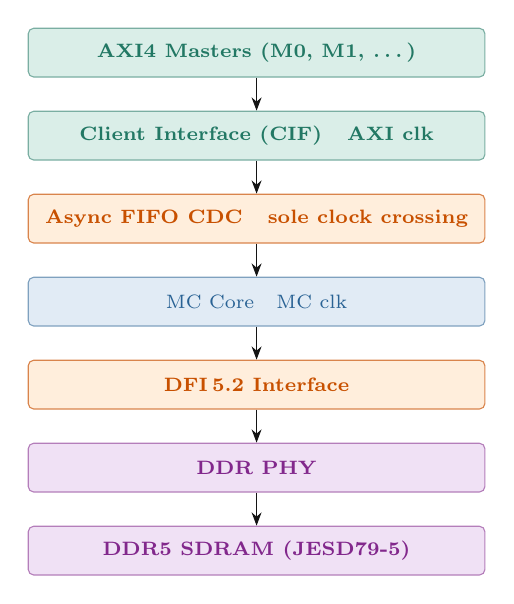
\begin{tikzpicture}[node distance=0.42cm and 0cm]
  \node[tblk,minimum width=5.8cm]  (axi) {AXI4 Masters (M0, M1, \ldots)};
  \node[tblk,minimum width=5.8cm,below=of axi]  (cif) {Client Interface (CIF)\quad AXI clk};
  \node[amblk,minimum width=5.8cm,below=of cif] (cdc) {Async FIFO CDC\quad sole clock crossing};
  \node[ablk,minimum width=5.8cm,below=of cdc]  (mc)  {MC Core\quad MC clk};
  \node[amblk,minimum width=5.8cm,below=of mc]  (dfi) {DFI\,5.2 Interface};
  \node[pblk,minimum width=5.8cm,below=of dfi]  (phy) {DDR PHY};
  \node[pblk,minimum width=5.8cm,below=of phy]  (ddr) {DDR5 SDRAM (JESD79-5)};

  \foreach \a/\b in {axi/cif,cif/cdc,cdc/mc,mc/dfi,dfi/phy,phy/ddr}
    \draw[arr] (\a)--(\b);
\end{tikzpicture}
\caption{Full system hierarchy. Teal = CIF/AXI. Blue = MC Core. Amber = clock crossing
         / DFI boundary. Purple = PHY + DRAM.}
\end{figure}

\subsection{System Scope Decisions (ADR-0000)}

\begin{center}
\begin{tabularx}{\linewidth}{@{} l l X @{}}
\toprule
\Th{Parameter} & \Th{Type} & \Th{Value / Options} \\
\midrule
\RA DDR Generation   & Compile-time & DDR5 (JESD79-5) \\
\RB Device Width     & Compile-time & x4 / x8 / x16 --- \textcolor{acc2}{\textbf{OPEN: ISSUE-0001}} \\
\RA Density          & Compile-time & 8\,Gb / 16\,Gb / 32\,Gb / 64\,Gb --- \textcolor{acc2}{\textbf{OPEN}} \\
\RB Rank Count       & Compile-time & Single / Multi --- \textcolor{acc2}{\textbf{OPEN: ISSUE-0002}} \\
\RA Topology         & Compile-time & Discrete / UDIMM / SODIMM --- \textcolor{acc2}{\textbf{OPEN}} \\
\RB DFI Version      & Compile-time & DFI\,5.2 \\
\RA Page Policy      & Runtime      & Open / Closed / Adaptive \\
\RB Refresh Policy   & Runtime      & REFab / REFsb / FGR --- \textcolor{acc2}{\textbf{OPEN: ISSUE-0003}} \\
\RA Timing Values    & Runtime      & All tXX from Config Registers \\
\RB RFM Parameters   & Runtime      & RAAIMT, RAAMMT, RAADec --- \textcolor{acc2}{\textbf{OPEN: ISSUE-0004}} \\
\RA DFI Freq Ratio   & Runtime      & 1:1, 1:2, 1:4 --- \textcolor{acc2}{\textbf{OPEN: ISSUE-0005}} \\
\bottomrule
\end{tabularx}
\end{center}

%%%%%%%%%%%%%%%%%%%%%%%%%%%%%%%%%%%%%%%%%%%%%%%%%%%%%%%%%%%%%%%%%%%%%%%%%%%%
\section{Architecture Completeness}
%%%%%%%%%%%%%%%%%%%%%%%%%%%%%%%%%%%%%%%%%%%%%%%%%%%%%%%%%%%%%%%%%%%%%%%%%%%%

\subsection{Per-Domain Completion}

\begin{center}
\begin{tabularx}{\linewidth}{@{} l r l X @{}}
\toprule
\Th{Domain} & \Th{\%} & \Th{Status} & \Th{Biggest Gap} \\
\midrule
\RA Requirements / JEDEC       & 80\% & \textcolor{acc3}{\textbf{Good}}    & Bank organisation vs device width \\
\RB CIF Architecture           & 35\% & \textcolor{acc2}{\textbf{Partial}} & Command format, CDC contract, queue architecture \\
\RA CDC Architecture           & 15\% & \textcolor{critbdr}{\textbf{Weak}} & Depth, backpressure, reset, overflow \\
\RB MC Core                    & 65\% & \textcolor{acc3}{\textbf{Solid}}   & Rank Manager, Maintenance Arbiter, DFI ownership \\
\RA DFI Interface              & 10\% & \textcolor{critbdr}{\textbf{Weak}} & All six sub-interfaces unspecified \\
\RB PHY Architecture           &  0\% & \textcolor{critbdr}{\textbf{None}} & Everything \\
\RA Verification Architecture  &  0\% & \textcolor{critbdr}{\textbf{None}} & Everything \\
\midrule
\RA \textbf{Overall}           & \textbf{$\approx$40\%} & \textcolor{acc2}{\textbf{Architecture Phase}} & --- \\
\bottomrule
\end{tabularx}
\end{center}

\subsection{Progress Bars}

\begin{center}
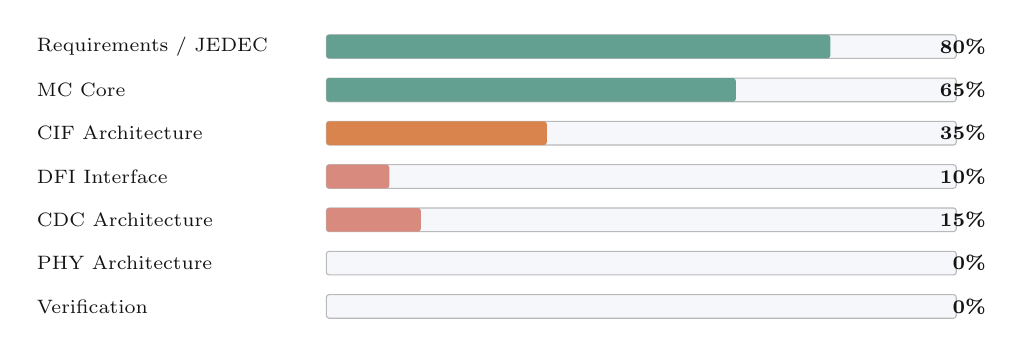
\begin{tikzpicture}
  % Requirements/JEDEC 80%
  \fill[boxfill,draw=ruleclr,rounded corners=1pt] (0,0.04) rectangle (8.0,0.34);
  \fill[acc3!70,rounded corners=1pt] (0,0.04) rectangle (6.4,0.34);
  \node[anchor=west,font=\scriptsize,text=hdrclr] at (-3.8,0.19) {Requirements / JEDEC};
  \node[anchor=east,font=\scriptsize\bfseries,text=hdrclr] at (8.5,0.19) {80\%};
  % MC Core 65%
  \fill[boxfill,draw=ruleclr,rounded corners=1pt] (0,-0.51) rectangle (8.0,-0.21);
  \fill[acc3!70,rounded corners=1pt] (0,-0.51) rectangle (5.2,-0.21);
  \node[anchor=west,font=\scriptsize,text=hdrclr] at (-3.8,-0.36) {MC Core};
  \node[anchor=east,font=\scriptsize\bfseries,text=hdrclr] at (8.5,-0.36) {65\%};
  % CIF 35%
  \fill[boxfill,draw=ruleclr,rounded corners=1pt] (0,-1.06) rectangle (8.0,-0.76);
  \fill[acc2!70,rounded corners=1pt] (0,-1.06) rectangle (2.8,-0.76);
  \node[anchor=west,font=\scriptsize,text=hdrclr] at (-3.8,-0.91) {CIF Architecture};
  \node[anchor=east,font=\scriptsize\bfseries,text=hdrclr] at (8.5,-0.91) {35\%};
  % DFI 10%
  \fill[boxfill,draw=ruleclr,rounded corners=1pt] (0,-1.61) rectangle (8.0,-1.31);
  \fill[critbdr!60,rounded corners=1pt] (0,-1.61) rectangle (0.8,-1.31);
  \node[anchor=west,font=\scriptsize,text=hdrclr] at (-3.8,-1.46) {DFI Interface};
  \node[anchor=east,font=\scriptsize\bfseries,text=hdrclr] at (8.5,-1.46) {10\%};
  % CDC 15%
  \fill[boxfill,draw=ruleclr,rounded corners=1pt] (0,-2.16) rectangle (8.0,-1.86);
  \fill[critbdr!60,rounded corners=1pt] (0,-2.16) rectangle (1.2,-1.86);
  \node[anchor=west,font=\scriptsize,text=hdrclr] at (-3.8,-2.01) {CDC Architecture};
  \node[anchor=east,font=\scriptsize\bfseries,text=hdrclr] at (8.5,-2.01) {15\%};
  % PHY 0%
  \fill[boxfill,draw=ruleclr,rounded corners=1pt] (0,-2.71) rectangle (8.0,-2.41);
  \node[anchor=west,font=\scriptsize,text=hdrclr] at (-3.8,-2.56) {PHY Architecture};
  \node[anchor=east,font=\scriptsize\bfseries,text=hdrclr] at (8.5,-2.56) {0\%};
  % Verification 0%
  \fill[boxfill,draw=ruleclr,rounded corners=1pt] (0,-3.26) rectangle (8.0,-2.96);
  \node[anchor=west,font=\scriptsize,text=hdrclr] at (-3.8,-3.11) {Verification};
  \node[anchor=east,font=\scriptsize\bfseries,text=hdrclr] at (8.5,-3.11) {0\%};
\end{tikzpicture}
\end{center}

%%%%%%%%%%%%%%%%%%%%%%%%%%%%%%%%%%%%%%%%%%%%%%%%%%%%%%%%%%%%%%%%%%%%%%%%%%%%
\section{What Is Defined}
%%%%%%%%%%%%%%%%%%%%%%%%%%%%%%%%%%%%%%%%%%%%%%%%%%%%%%%%%%%%%%%%%%%%%%%%%%%%

\subsection{MC Core --- Defined Blocks}

\begin{center}
\begin{tabularx}{\linewidth}{@{} l l X @{}}
\toprule
\Th{Block} & \Th{Status} & \Th{Coverage} \\
\midrule
\RA Config Registers    & Defined & Full register table (32+ regs), all timing params \\
\RB Init FSM            & Defined & 16-state sequence, MRW burst, ZQCAL, DLL reset \\
\RA Bank State Machines & Defined & 11 states, 16 instances, all per-bank timers \\
\RB Timing Control      & Defined & All cross-bank constraints, tFAW window, countdown timers \\
\RA Arbitration Logic   & Defined & 6-level priority, age counters, watermark switching \\
\RB Command Selector    & Defined & Page policy, BG-aware reorder, 16-gate legal check matrix \\
\RA Refresh Scheduler   & Defined & REFab, REFsb, FGR, leaky-bucket, urgent override \\
\RB ZQcal FSM           & Defined & MPC ZQCAL Start/Latch flow, periodic interval \\
\RA RFM FSM             & Defined & Per-bank RAA counters, RAAIMT threshold, tRFM \\
\RB Power Management    & Defined & Precharge PD, Active PD, Self-Refresh, MPSM \\
\RA Write Data Path     & Defined & BL16 buffer, DM/ECC, Write CRC, WL align, DFI timing \\
\RB Read Data Path      & Defined & Latency counter, data FIFO, ECC/CRC checker, ECS FSM \\
\bottomrule
\end{tabularx}
\end{center}

\subsection{CIF --- Defined Blocks}

\begin{center}
\begin{tabularx}{\linewidth}{@{} l l X @{}}
\toprule
\Th{Block} & \Th{Status} & \Th{Coverage} \\
\midrule
\RA AXI Write Port       & Partial & AW/W channel handlers, B-response generator \\
\RB AXI Read Port        & Partial & AR channel, outstanding request tracking \\
\RA Burst Splitter       & Partial & Page boundary split (Stage 1), BL alignment (Stage 2) \\
\RB Address Translator   & Partial & Bit-field extractor, CMD builder, configurable mapping \\
\RA Write Cmd Pool       & Partial & Entry storage, allocation, dispatch identified \\
\RB Read Cmd Pool        & Partial & Entry storage, allocation, dispatch identified \\
\RA Reorder Buffer (ROB) & Partial & Per-AXID queues, seqnum tagging, HEAD retirement \\
\RB Merge Logic          & Partial & Fragment buffer, reassembly tracker, output mux \\
\RA Response Tracking    & Partial & Seqnum generator, tag insertion, tag lookup \\
\bottomrule
\end{tabularx}
\end{center}

%%%%%%%%%%%%%%%%%%%%%%%%%%%%%%%%%%%%%%%%%%%%%%%%%%%%%%%%%%%%%%%%%%%%%%%%%%%%
\section{Critical Issues}
%%%%%%%%%%%%%%%%%%%%%%%%%%%%%%%%%%%%%%%%%%%%%%%%%%%%%%%%%%%%%%%%%%%%%%%%%%%%

\begin{critbox}{CRITICAL-1 --- Bank Organisation Inconsistency}
Documents assume \textbf{16 banks (2\,BG $\times$ 4\,banks $\times$ 2 sub-channels)}.

DDR5 actual organisation:
\begin{itemize}
  \item x4/x8 devices: 8\,BG $\times$ 4\,banks = \textbf{32 banks}
  \item x16 devices: 4\,BG $\times$ 4\,banks = \textbf{16 banks}
\end{itemize}
\textbf{Impact:} Address Mapper, Bank FSM count, Refresh Scheduler, all timing formulae.\\
\textbf{Resolution:} Answer ISSUE-0001 (target device width + density) before any RTL.
\end{critbox}

\vspace{4pt}
\begin{critbox}{CRITICAL-2 --- Missing Rank Manager}
Rank state is currently scattered across Refresh Scheduler, Power FSM, and Timing Control.

Required dedicated block owning:
\texttt{rank\_busy}, \texttt{rank\_refresh}, \texttt{rank\_power\_state},
\texttt{rank\_self\_refresh}, \texttt{rank\_zq\_block}, \texttt{rank\_cke}

\textbf{Impact:} DFI integration will be painful without a single rank state source of truth.
\end{critbox}

\vspace{4pt}
\begin{critbox}{CRITICAL-3 --- Missing Maintenance Arbiter}
REF, RFM, ZQ, MRR, and Scrubber run independently with no defined collision behaviour.

Scenario: \texttt{ref\_urgent} + \texttt{rfm\_trigger} + \texttt{zq\_expiry} same cycle.

Required: \textbf{Maintenance Arbiter} with explicit priority and mutual-exclusion rules.\\
Required document: \texttt{Maintenance\_Arbiter.md}
\end{critbox}

\vspace{4pt}
\begin{critbox}{CRITICAL-4 --- DFI Training Ownership Undefined}
\texttt{TRAINING\_DISPATCH} exists inside Init FSM but ownership boundary is undefined.

Required separation:
\begin{itemize}
  \item MC owns: sequencing, handshake signals, retry logic
  \item PHY owns: execution, measurement, result reporting
  \item DFI owns: handshake protocol (\texttt{dfi\_wrlvl\_en/resp}, \texttt{dfi\_rdlvl\_en/resp})
\end{itemize}
Required document: \texttt{DFI\_Training\_Orchestrator.md}
\end{critbox}

\vspace{4pt}
\begin{warnbox}{ARCH-1 --- Duplicate Queue Structure Risk}
CIF contains Write Cmd Pool and Read Cmd Pool.\\
MC Core also referenced RD/WR pools downstream of CDC.

\textbf{Option A (correct):} CIF Pools $\to$ CDC $\to$ MC Scheduler (no duplicate queuing)\\
\textbf{Option B (incorrect):} CIF Pools $\to$ CDC $\to$ MC Pools $\to$ Scheduler (extra latency, extra storage)

\textbf{Resolution required in ADR-0004.}
\end{warnbox}

\vspace{4pt}
\begin{warnbox}{ARCH-2 --- Address Mapper has No Owner}
Physical address $\to$ Channel $\to$ Rank $\to$ BG $\to$ Bank $\to$ Row $\to$ Column
mapping is referenced in CIF and Config Registers but owned by neither.

Required: explicit \textbf{Address Mapper} block between Burst Splitter and Cmd Pools.\\
Required document: \texttt{Address\_Mapping.md}
\end{warnbox}

\vspace{4pt}
\begin{warnbox}{ARCH-3 --- Missing Command Queue Architecture}
Command entry format, depth, allocation, retirement, hazards, reordering limits, and
age counter details are unspecified.\\
Required document: \texttt{Command\_Queue\_Architecture.md}
\end{warnbox}

%%%%%%%%%%%%%%%%%%%%%%%%%%%%%%%%%%%%%%%%%%%%%%%%%%%%%%%%%%%%%%%%%%%%%%%%%%%%
\section{What Is Missing}
%%%%%%%%%%%%%%%%%%%%%%%%%%%%%%%%%%%%%%%%%%%%%%%%%%%%%%%%%%%%%%%%%%%%%%%%%%%%

\subsection{MC Core --- Missing Blocks}

\begin{center}
\begin{tabularx}{\linewidth}{@{} l l X @{}}
\toprule
\Th{Block} & \Th{Priority} & \Th{Reason Needed} \\
\midrule
\RC Rank Manager         & P0 --- Critical & Single source of truth for all rank state; required before DFI integration \\
\RC Maintenance Arbiter  & P0 --- Critical & Collision arbitration for REF/RFM/ZQ/MRR/Scrub \\
\RC DFI Training Orchestrator & P0 --- Critical & Training ownership boundary between MC, DFI, PHY \\
\RC Address Mapper       & P0 --- Critical & Physical $\to$ \{channel, rank, BG, bank, row, col\} \\
\RB Command Queue Spec   & P1 --- High & Entry format, depth, hazards, retirement rules \\
\RB CDC Contract         & P1 --- High & FIFO depth, backpressure, overflow, underflow, reset \\
\RB Statistics Block     & P2 & row\_hits, misses, BG conflicts, read/write latency \\
\RB Performance Monitor  & P2 & Cmds issued, refresh count, stall cycles, bank utilisation \\
\RB Debug Architecture   & P2 & Trace buffer, event log, status registers \\
\RB Error Architecture   & P2 & ECC, CRC, training failures, refresh violations \\
\RB Interrupt Controller & P2 & init\_done, training\_done, ecc\_error, fatal\_error \\
\bottomrule
\end{tabularx}
\end{center}

\subsection{CIF --- Missing Documents}

\begin{center}
\begin{tabularx}{\linewidth}{@{} l l @{}}
\toprule
\Th{Document} & \Th{Blocks It Resolves} \\
\midrule
\RA \texttt{CIF\_Architecture.pdf}         & Full CIF decomposition and interfaces \\
\RB \texttt{Address\_Mapping.pdf}          & Field extraction, configurable bit-mapping, DDR3/4/5 support \\
\RA \texttt{Burst\_Splitter.pdf}           & Stage 1 (page boundary), Stage 2 (BL alignment), math \\
\RB \texttt{Write\_Cmd\_Pool.pdf}          & Entry format, depth, allocation, dispatch, free \\
\RA \texttt{Read\_Cmd\_Pool.pdf}           & Same as write \\
\RB \texttt{Response\_Tracking.pdf}        & Seqnum generator, tag format, lookup \\
\RA \texttt{Reorder\_Buffer.pdf}           & Per-AXID queues, HEAD retirement, isolation guarantees \\
\RB \texttt{Merge\_Logic.pdf}              & Fragment buffer, reassembly, bypass path \\
\bottomrule
\end{tabularx}
\end{center}

\subsection{DFI Interface --- Missing Sub-Interfaces}

\begin{center}
\begin{tabularx}{\linewidth}{@{} l X @{}}
\toprule
\Th{Sub-Interface} & \Th{Status} \\
\midrule
\RA Command Interface   & Partially mapped (address/bank/bg/cs signals in MC doc) \\
\RB Read Path           & rddata, rddata\_valid, rddata\_en, rddata\_dnv \\
\RA Write Path          & wrdata, wrdata\_mask, wrdata\_en, wrdata\_cs\_n, parity \\
\RB Update Interface    & ctrlupd\_req/ack, phyupd\_req/ack --- undefined ownership \\
\RA Training Interface  & wrlvl\_en/strobe, rdlvl\_en/resp, calvl\_en --- undefined \\
\RB Low Power Interface & cke, cksre/srx, init\_start/complete --- partially mapped \\
\bottomrule
\end{tabularx}
\end{center}

%%%%%%%%%%%%%%%%%%%%%%%%%%%%%%%%%%%%%%%%%%%%%%%%%%%%%%%%%%%%%%%%%%%%%%%%%%%%
\section{Obsidian Knowledge Graph}
%%%%%%%%%%%%%%%%%%%%%%%%%%%%%%%%%%%%%%%%%%%%%%%%%%%%%%%%%%%%%%%%%%%%%%%%%%%%

\subsection{Root Graph Structure}

\begin{figure}[h]
\centering
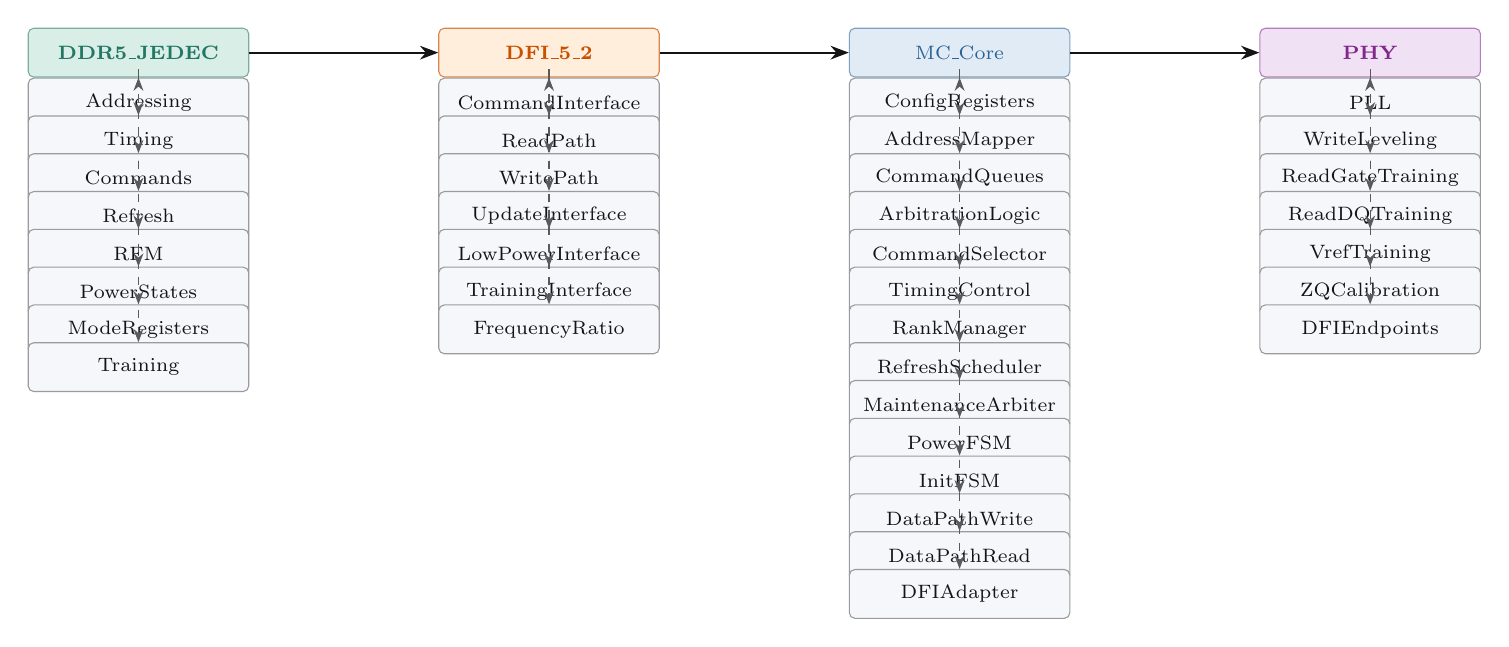
\begin{tikzpicture}[node distance=0.38cm and 1.4cm]

  %% Column 1: JEDEC
  \node[tblk,minimum width=2.8cm] (jedec) {DDR5\_JEDEC};
  \foreach \lbl/\i in {Addressing/1,Timing/2,Commands/3,Refresh/4,
                       RFM/5,PowerStates/6,ModeRegisters/7,Training/8}{
    \node[mblk,minimum width=2.8cm,below=\i*0.48cm of jedec.south,
          yshift=0.48cm,anchor=north] (j\i) {\lbl};
    \draw[darr] (jedec.south) -- (j\i.north);
  }

  %% Column 2: DFI
  \node[amblk,minimum width=2.8cm,right=2.4cm of jedec] (dfi) {DFI\_5\_2};
  \foreach \lbl/\i in {CommandInterface/1,ReadPath/2,WritePath/3,
                       UpdateInterface/4,LowPowerInterface/5,
                       TrainingInterface/6,FrequencyRatio/7}{
    \node[mblk,minimum width=2.8cm,below=\i*0.48cm of dfi.south,
          yshift=0.48cm,anchor=north] (d\i) {\lbl};
    \draw[darr] (dfi.south) -- (d\i.north);
  }

  %% Column 3: MC Core
  \node[ablk,minimum width=2.8cm,right=2.4cm of dfi] (mc) {MC\_Core};
  \foreach \lbl/\i in {ConfigRegisters/1,AddressMapper/2,CommandQueues/3,
                       ArbitrationLogic/4,CommandSelector/5,TimingControl/6,
                       RankManager/7,RefreshScheduler/8,MaintenanceArbiter/9,
                       PowerFSM/10,InitFSM/11,DataPathWrite/12,
                       DataPathRead/13,DFIAdapter/14}{
    \node[mblk,minimum width=2.8cm,below=\i*0.48cm of mc.south,
          yshift=0.48cm,anchor=north] (m\i) {\lbl};
    \draw[darr] (mc.south) -- (m\i.north);
  }

  %% Column 4: PHY
  \node[pblk,minimum width=2.8cm,right=2.4cm of mc] (phy) {PHY};
  \foreach \lbl/\i in {PLL/1,WriteLeveling/2,ReadGateTraining/3,
                       ReadDQTraining/4,VrefTraining/5,
                       ZQCalibration/6,DFIEndpoints/7}{
    \node[mblk,minimum width=2.8cm,below=\i*0.48cm of phy.south,
          yshift=0.48cm,anchor=north] (p\i) {\lbl};
    \draw[darr] (phy.south) -- (p\i.north);
  }

  %% Top-level arrows
  \draw[arr,thick] (jedec.east)--(dfi.west);
  \draw[arr,thick] (dfi.east)--(mc.west);
  \draw[arr,thick] (mc.east)--(phy.west);

\end{tikzpicture}
\caption{Obsidian root knowledge graph. Each column is a top-level node; children are
         sub-topic notes. Arrows show dependency direction (JEDEC $\to$ DFI $\to$ MC $\to$ PHY).}
\end{figure}

\subsection{CIF Sub-Graph}

\begin{center}
\begin{tabularx}{\linewidth}{@{} l l @{}}
\toprule
\Th{CIF Node} & \Th{Child Nodes} \\
\midrule
\RA AXI\_Write\_Port & AW\_Channel\_Handler, W\_Channel\_Handler, Write\_Request\_Validation, B\_Response\_Generator \\
\RB AXI\_Read\_Port  & AR\_Channel\_Handler, Read\_Request\_Validation, Outstanding\_Request\_Tracking, Read\_Request\_Formatter \\
\RA Burst\_Splitter  & Page\_Boundary\_Detector, Burst\_Split\_Logic, Command\_Generator, Metadata\_Generator \\
\RB Address\_Translator & Address\_Mapping, Field\_Extractor, Mapping\_Config, Address\_Validation \\
\RA Write\_Cmd\_Pool & Entry\_Storage, Allocation, Dispatch, Free \\
\RB Read\_Cmd\_Pool  & Entry\_Storage, Allocation, Dispatch, Free \\
\RA Response\_Tracking & Sequence\_Number\_Generator, Tag\_Generator, Attribute\_Buffer, Tag\_Lookup \\
\RB Reorder\_Buffer  & Per\_AXID\_Queues, Fill, Ordering, Retirement \\
\RA Merge\_Logic     & Response\_Collection, Burst\_Reconstruction, Response\_Merge, AXI\_Response\_Formatter \\
\bottomrule
\end{tabularx}
\end{center}

%%%%%%%%%%%%%%%%%%%%%%%%%%%%%%%%%%%%%%%%%%%%%%%%%%%%%%%%%%%%%%%%%%%%%%%%%%%%
\section{Architecture Decision Records (ADR)}
%%%%%%%%%%%%%%%%%%%%%%%%%%%%%%%%%%%%%%%%%%%%%%%%%%%%%%%%%%%%%%%%%%%%%%%%%%%%

\subsection{Completed ADRs}

\begin{center}
\begin{tabularx}{\linewidth}{@{} l l X @{}}
\toprule
\Th{ADR} & \Th{Title} & \Th{Decision} \\
\midrule
\RA ADR-0000  & System Scope        & Compile-time: DDR gen, width, density, rank, DFI version. Runtime: policy, timing, RFM. \\
\RB ADR-0000A & Config Model        & Boot-time configurable vs runtime. Requires-reset and requires-retraining flags defined. \\
\RA ADR-0000B & Ownership Matrix    & All 14 MC Core blocks + CIF blocks assigned explicit ownership. \\
\RB ADR-0000C & Context Objects     & Bank Context, Rank Context, Command Context, Refresh Context all defined. \\
\bottomrule
\end{tabularx}
\end{center}

\subsection{Required ADRs --- Priority 0}

\begin{center}
\begin{tabularx}{\linewidth}{@{} l l X @{}}
\toprule
\Th{ADR} & \Th{Title} & \Th{Blocks on This} \\
\midrule
\RC ADR-0001 & Command Format      & Queue depth, entry fields, tag format, allocation, retirement \\
\RC ADR-0002 & Address Mapping     & Physical $\to$ \{channel, rank, BG, bank, row, col\}; configurable bit-field scheme \\
\RC ADR-0003 & CDC Contract        & FIFO depth, backpressure protocol, overflow/underflow, reset strategy \\
\RC ADR-0004 & Queue Architecture  & CIF pool vs MC pool decision (Option A vs B); hazard rules; reordering limits \\
\RC ADR-0005 & Command Lifecycle   & Allocation $\to$ dispatch $\to$ issue $\to$ completion $\to$ retirement state machine \\
\RC ADR-0006 & Timing Ownership    & Which block owns which constraint timer; cross-block update protocol \\
\bottomrule
\end{tabularx}
\end{center}

\subsection{Required ADRs --- Priority 1}

\begin{center}
\begin{tabularx}{\linewidth}{@{} l l X @{}}
\toprule
\Th{ADR} & \Th{Title} & \Th{Blocks on This} \\
\midrule
\RB ADR-0007 & Rank Manager        & rank\_busy, rank\_refresh, rank\_power, rank\_sr, rank\_zq --- all signals \\
\RA ADR-0008 & Maintenance Arbiter & Priority order for REF/RFM/ZQ/MRR/Scrub collision resolution \\
\RB ADR-0009 & Training Architecture & MC/DFI/PHY boundary; write leveling; read gate; DQ; VREF; CA; CS \\
\RA ADR-0010 & DFI Ownership       & Which MC sub-block drives which DFI signal; timing adapters \\
\bottomrule
\end{tabularx}
\end{center}

\subsection{Required ADRs --- Priority 2}

\begin{center}
\begin{tabularx}{\linewidth}{@{} l l @{}}
\toprule
\Th{ADR} & \Th{Title} \\
\midrule
\RA ADR-0011 & PHY Architecture (PLL, clocking, read/write paths, calibration) \\
\RB ADR-0012 & Verification Architecture (coverage model, assertions, scoreboards, compliance) \\
\bottomrule
\end{tabularx}
\end{center}

%%%%%%%%%%%%%%%%%%%%%%%%%%%%%%%%%%%%%%%%%%%%%%%%%%%%%%%%%%%%%%%%%%%%%%%%%%%%
\section{Open Issues Register}
%%%%%%%%%%%%%%%%%%%%%%%%%%%%%%%%%%%%%%%%%%%%%%%%%%%%%%%%%%%%%%%%%%%%%%%%%%%%

\begin{center}
\begin{tabularx}{\linewidth}{@{} l l l X @{}}
\toprule
\Th{ID} & \Th{Title} & \Th{Status} & \Th{Impacts} \\
\midrule
\RC ISSUE-0001 & Target DRAM Organisation & \textcolor{critbdr}{\textbf{OPEN}} &
  Bank count, Address Mapper, BSM instances, Refresh Scheduler \\
\RC ISSUE-0002 & Single vs Multi Rank     & \textcolor{critbdr}{\textbf{OPEN}} &
  Refresh, Power Management, Training, DFI per-rank signals \\
\RC ISSUE-0003 & Refresh Strategy         & \textcolor{critbdr}{\textbf{OPEN}} &
  REFab vs REFsb vs hybrid; FGR mode; tRFCsb in BSM \\
\RC ISSUE-0004 & RFM Support Level        & \textcolor{critbdr}{\textbf{OPEN}} &
  Mandatory/optional/disabled; RAAIMT/RAAMMT register fields \\
\RC ISSUE-0005 & DFI Frequency Ratio      & \textcolor{critbdr}{\textbf{OPEN}} &
  1:1/1:2/1:4; all DFI timing formulae depend on this \\
\RB ISSUE-0006 & PHY Ownership Boundary   & \textcolor{acc2}{\textbf{OPEN}} &
  Which signals MC drives vs PHY drives at DFI boundary \\
\RA ISSUE-0007 & CIF Duplicate Queue Risk & \textcolor{acc2}{\textbf{OPEN}} &
  Option A vs B; resolves in ADR-0004 \\
\bottomrule
\end{tabularx}
\end{center}

%%%%%%%%%%%%%%%%%%%%%%%%%%%%%%%%%%%%%%%%%%%%%%%%%%%%%%%%%%%%%%%%%%%%%%%%%%%%
\section{Context Objects}
%%%%%%%%%%%%%%%%%%%%%%%%%%%%%%%%%%%%%%%%%%%%%%%%%%%%%%%%%%%%%%%%%%%%%%%%%%%%

\begin{center}
\begin{tabularx}{\linewidth}{@{} l X @{}}
\toprule
\Th{Context} & \Th{Fields} \\
\midrule
\RA Bank Context &
  \texttt{bank\_state}, \texttt{open\_row}, \texttt{active\_row},
  \texttt{tRCD}, \texttt{tRAS}, \texttt{tRP}, \texttt{tRFC} \\
\RB Rank Context &
  \texttt{rank\_state}, \texttt{refresh\_state}, \texttt{power\_state},
  \texttt{zq\_state} \\
\RA Command Context &
  \texttt{command\_id}, \texttt{axi\_id}, \texttt{rank}, \texttt{bg},
  \texttt{bank}, \texttt{row}, \texttt{column}, \texttt{priority},
  \texttt{age}, \texttt{timestamp} \\
\RB Refresh Context &
  \texttt{credits}, \texttt{last\_refresh}, \texttt{urgent\_flag},
  \texttt{mode} (REFab/REFsb/FGR) \\
\bottomrule
\end{tabularx}
\end{center}

%%%%%%%%%%%%%%%%%%%%%%%%%%%%%%%%%%%%%%%%%%%%%%%%%%%%%%%%%%%%%%%%%%%%%%%%%%%%
\section{Ownership Matrix}
%%%%%%%%%%%%%%%%%%%%%%%%%%%%%%%%%%%%%%%%%%%%%%%%%%%%%%%%%%%%%%%%%%%%%%%%%%%%

\begin{center}
\begin{tabularx}{\linewidth}{@{} l l l X @{}}
\toprule
\Th{Block} & \Th{Layer} & \Th{State} & \Th{Interfaces} \\
\midrule
\RA AXI Write/Read Port  & CIF & Partial & AXI AW/W/AR/B/R channels \\
\RB Burst Splitter       & CIF & Partial & AXI burst $\to$ sub-transactions \\
\RA Address Translator   & CIF & Partial & byte\_addr $\to$ \{rank, BG, bank, row, col\} \\
\RB Cmd Pools (WR/RD)    & CIF & Partial & Accepts from translator; drives CDC \\
\RA Reorder Buffer       & CIF & Partial & Tags, per-AXID queue, HEAD retirement \\
\RB Merge Logic          & CIF & Partial & Fragment reassembly, ROB feed \\
\RA Async FIFO CDC       & CDC & Weak   & AXI clk $\to$ MC clk crossing \\
\RB Config Registers     & MC  & Defined & APB/CSR slave, all timing params \\
\RA Init FSM             & MC  & Defined & DFI direct; INIT\_KICK $\to$ init\_done \\
\RB Bank State Machines  & MC  & Defined & 16 instances; per-bank timers \\
\RA Timing Control       & MC  & Defined & \texttt{cmd\_ok[15:0][cmd\_type]} per cycle \\
\RB Arbitration Logic    & MC  & Defined & Priority, age, watermark; winner class \\
\RA Command Selector     & MC  & Defined & Legal check, page policy, sequence gen \\
\RB Refresh Scheduler    & MC  & Defined & REFab/REFsb, FGR, leaky-bucket \\
\RA ZQcal FSM            & MC  & Defined & MPC ZQCAL Start/Latch \\
\RB RFM FSM              & MC  & Defined & RAA per bank, RAAIMT threshold \\
\RA Power Mgmt FSM       & MC  & Defined & PD, SR, MPSM transitions \\
\RB Write Data Path      & MC  & Defined & BL16 buffer, CRC, WL align, DFI write \\
\RA Read Data Path       & MC  & Defined & Latency counter, CRC checker, ECS FSM \\
\RB \textcolor{critbdr}{Rank Manager}        & MC & \textcolor{critbdr}{MISSING} & rank\_busy, rank\_cke, rank\_sr --- all rank signals \\
\RA \textcolor{critbdr}{Maintenance Arbiter} & MC & \textcolor{critbdr}{MISSING} & Collision resolution for REF/RFM/ZQ/MRR \\
\RB \textcolor{critbdr}{Address Mapper}      & MC & \textcolor{critbdr}{MISSING} & Physical addr decomposition \\
\RA \textcolor{critbdr}{DFI Training Orch.}  & MC & \textcolor{critbdr}{MISSING} & Training handshake boundary \\
\RB \textcolor{critbdr}{DFI Adapter}         & MC & \textcolor{critbdr}{Weak}    & Signal encoding, freq ratio, latency \\
\bottomrule
\end{tabularx}
\end{center}

%%%%%%%%%%%%%%%%%%%%%%%%%%%%%%%%%%%%%%%%%%%%%%%%%%%%%%%%%%%%%%%%%%%%%%%%%%%%
\section{Verification Coverage Nodes Required}
%%%%%%%%%%%%%%%%%%%%%%%%%%%%%%%%%%%%%%%%%%%%%%%%%%%%%%%%%%%%%%%%%%%%%%%%%%%%

\begin{center}
\begin{tabularx}{\linewidth}{@{} l l X @{}}
\toprule
\Th{Document} & \Th{Status} & \Th{Coverage Model} \\
\midrule
\RA \texttt{Coverage\_BankFSM.md}     & Not started & All 11 states, all transitions, illegal transition exclusions \\
\RB \texttt{Coverage\_Refresh.md}     & Not started & REFab, REFsb, FGR, credit max, urgent stall, derating \\
\RA \texttt{Coverage\_Turnaround.md}  & Not started & tWTR\_L/S, tRTW, BG hit/miss combinations \\
\RB \texttt{Coverage\_RFM.md}         & Not started & RAA increment, decrement, threshold hit, RFM injection \\
\RA \texttt{Coverage\_DFI.md}         & Not started & All 6 DFI sub-interfaces, latency correctness \\
\RB \texttt{Coverage\_Training.md}    & Not started & WL, read gate, DQ, VREF, CA, CS training sequences \\
\RA \texttt{Coverage\_Powersave.md}   & Not started & PD entry/exit, SR entry/exit, MPSM, tXP, tXS, tDLLK \\
\bottomrule
\end{tabularx}
\end{center}

%%%%%%%%%%%%%%%%%%%%%%%%%%%%%%%%%%%%%%%%%%%%%%%%%%%%%%%%%%%%%%%%%%%%%%%%%%%%
\section{Time Estimate \& Roadmap}
%%%%%%%%%%%%%%%%%%%%%%%%%%%%%%%%%%%%%%%%%%%%%%%%%%%%%%%%%%%%%%%%%%%%%%%%%%%%

\subsection{Assumptions}

1 person, part-time, ECE capstone level. Architecture first, RTL second.

\subsection{Phase Estimates}

\begin{center}
\begin{tabularx}{\linewidth}{@{} l l r X @{}}
\toprule
\Th{Phase} & \Th{Milestone} & \Th{Time} & \Th{Exit Criteria} \\
\midrule
\RA Architecture Completion & ADR-0001 through ADR-0006 done & 2--3 weeks &
  Architecture Freeze v1.0 signed off \\
\RB Architecture (P1) & ADR-0007 through ADR-0010 & 1 week &
  Rank Mgr, Maint. Arbiter, Training, DFI owner defined \\
\RA CIF RTL & AXI $\to$ CDC handoff complete & 4--6 weeks &
  Simulation passing basic read/write burst \\
\RB MC Core RTL & Init FSM through DFI adapter & 6--10 weeks &
  All FSMs, timing gates, and scheduler RTL complete \\
\RA DFI + PHY Interface & DFI adapter to PHY handshake & 2--4 weeks &
  DFI training handshake functional \\
\RB Training RTL & WL + read gate + DQ + VREF + CA & 2--4 weeks &
  All training sub-sequences pass simulation \\
\RA Verification & UVM TB, scoreboards, coverage & 8--12 weeks &
  Coverage closure; DDR5 + DFI compliance \\
\midrule
\RA \textbf{Total (architecture-first)} & & \textbf{5--6 months} & Aligns with capstone roadmap \\
\RB \textbf{Total (RTL without arch)} & & \textbf{8--10 months} & Multiple redesigns expected \\
\bottomrule
\end{tabularx}
\end{center}

\subsection{Current Recommendation}

\begin{okbox}{Hold Architecture --- Do Not Start RTL}
Current architecture is approximately \textbf{40\% complete} toward RTL readiness.

Complete the following before writing any RTL:
\begin{enumerate}
  \item ADR-0001: Command Format
  \item ADR-0002: Address Mapping
  \item ADR-0003: CDC Contract
  \item ADR-0004: Queue Architecture (resolve Option A vs B)
  \item ADR-0005: Command Lifecycle
  \item ADR-0006: Timing Ownership
\end{enumerate}
After these six ADRs, architecture completeness will reach $\approx$60\%,
which is the minimum threshold to start CIF RTL safely.
\end{okbox}

\subsection{Priority Upload Queue}

Documents needed next, in priority order:

\begin{enumerate}
  \item CIF architecture spec
  \item AXI $\to$ command conversion detail
  \item Address mapping scheme
  \item DFI interface spec (all 6 sub-interfaces)
  \item PHY architecture
  \item Training architecture
  \item Refresh / RFM design detail
  \item Verification plan
\end{enumerate}

\vspace{10pt}
\noindent\color{acc1!40}\rule{\linewidth}{0.5pt}\\[2pt]
{\small\color{notetext}
RMC Architecture Planning Session --- Analysis Report.
JEDEC JESD79-5 (DDR5) / DFI\,5.2 / AXI4.
Architecture phase. RTL not started.
Next milestone: Architecture Freeze v1.0 after ADR-0001 through ADR-0006.}

\end{document}
